\documentclass[a4paper,12pt]{book}
\usepackage{CJKutf8}
\usepackage{titlesec}
\usepackage{graphicx} 
\usepackage{subfigure}
\usepackage{amsbsy}
\usepackage{amsmath}
\usepackage{amssymb}
\usepackage{array}
\usepackage[colorlinks,linkcolor=blue]{hyperref}
\usepackage{enumitem}
\usepackage{color}
\usepackage{fontspec}
\makeatletter
\color{black}
\let\default@color\current@color
\makeatother
\usepackage{pythonhighlight}
% \usepackage[hyperref, UTF8]{ctex}
\newtheorem{definition}{Definition}
\setmonofont{Monaco}

\begin{CJK*}{UTF8}{gbsn}
    %%*****************文本设置********************
    \RequirePackage{indentfirst}
    \setlength{\parindent}{2em}
    %% 行距
    \linespread{1.3}
    \selectfont
    % 页面顶行空白
    \setlength{\topskip}{5ex}
    % 段间距
    \setlength{\parskip}{1ex}
    %item 的缩进%
    \setlength{\itemindent}{2em}
    %%********************************************
    
    \begin{document}
    \title{Word2vec笔记}
    \author{Kevin}
    \date{2020-06-28}
    \maketitle

    \newpage
    \tableofcontents
    
    \chapter{Word2Vec基本数学内容}
\section{Sigmod 函数}
Sigmod函数通常在二分类中应用。它将样本映射后投影在[0, 1]范围内,对应样本所属的类的概率。函数表达式如下所示:
\begin{equation}
    f(x) = \frac{1}{1+e^{-x}}
\end{equation}

具体的讨论可以参见:

\href{http://blog.csdn.net/chunyun0716/article/details/51580342}{Logistic Function AND Softmax Function}

\section{贝叶斯公式}
\begin{equation}
    P(A|B) = \frac{P(B|A)P(A)}{P(B)}
\end{equation}

可以参见贝叶斯分类等一系列文章:
\begin{enumerate}
    \item \href{http://blog.csdn.net/chunyun0716/article/details/51031055}{朴素贝叶斯分类}
    \item \href{http://blog.csdn.net/chunyun0716/article/details/51058948}{朴素贝叶斯算法的后验概率最大化含义}
    \item \href{http://blog.csdn.net/chunyun0716/article/details/51111864}{朴素贝叶斯法的参数估计}
\end{enumerate}

\section{Huffman 树和Huffman编码}
下边这篇博客写的很详细了,这里简单引用一些基本知识:

\href{http://blog.csdn.net/shuangde800/article/details/7341289}{哈夫曼树}


定义哈夫曼树之前先说明几个与哈夫曼树有关的概念:

\textbf{路径}: 树中一个结点到另一个结点之间的分支构成这两个结点之间的路径。

\textbf{路径长度}:路径上的分枝数目称作路径长度。

\textbf{树的路径长度}:从树根到每一个结点的路径长度之和。

\textbf{结点的带权路径长度}:在一棵树中,如果其结点上附带有一个权值,通常把该结点的路径长度与该结点上的权值                                                     之积称为该结点的带权路径长度(weighted path length)

\textbf{树的带权路径长度}:如果树中每个叶子上都带有一个权值,
则把树中所有叶子的带权路径长度之和称为树的带权路径长度。

一般来说,用$n(n>0)$个带权值的叶子来构造二叉树,
限定二叉树中除了这n个叶子外只能出现度为2的结点。
那么符合这样条件的二叉树往往可构造出许多颗,
其中带权路径长度最小的二叉树就称为\textbf{哈夫曼树}或\textbf{最优二叉树}.

\textbf{通过哈夫曼树来构造的编码称为哈弗曼编码(huffman code)}
    \chapter{语言模型}
    语言模型可以分为文法型模型和统计语言模型。在实际应用中语言识别、手写体文字识别、机器翻译、键盘输入、信息检索等研究领域都用到了语言模型。文法型语言模型是人工编制的语言学文法,文法规则来源于语言学家掌握的语言学知识和领域知识,但这种语言模型不能处理大规模真实文本。因此,统计语言模型出现了,并且得到了广泛的应用,统计语言模型是基于概率的,包括了N元文法模型(N-gram Model)、隐马尔科夫模型(Hidden Markov Model,简称HMM)、最大熵模型(Maximum Entropy Model)。

    \section{统计语言模型的基本原理}

    统计语言模型是以概率分布的形式说明了一个字符串出现的概率。
    假设词(word)是语言的最小单位,
    句子S是由一系列的词$w_1,w_2, \dots,w_k$顺序构成,
    则句子S的概率为下:
    \begin{equation}
        \begin{split}
            p(s) &= p(w_1)p(w_2|w_1)\dots p(w_n|w_1,w_2,\dots,w_{n-1}) \\
            &=\prod_{i=1}^{n}p(w_i|w_1,w_2,\dots,w_{i-1}) 
        \end{split}
    \end{equation}

    且,上式中约定$p(w_1|w_0)=p(w_1)$.观察上式可以发现,句子S的概率计算是很复杂的,因此,往往采用一些方法来估计语料库中句子的概率。

    \section{主要的统计语言模型}
    \subsection{上下文无关模型}
    上下文无关模型就是词$w_1$的出现与它所处的环境无关,仅仅是它在语料中出现的概率,即它是n-gram中n=1的情况,但是实际上,这种方法效果并不是很好。

    \subsection{n-gram模型}
    n-gram模型是要考虑上下文的。$w_1$出现的是依赖于它之前的n-1个词的,即需要计算词表中的每一个n-1元组的概率,此计算量是巨大的,因此实际中,常取n=2 或n=3.

    \chapter{Hierarchical Softmax模型}
    \section{词向量}
    词向量目前常用的有2种表示方法,One-hot representation 
    和 distributed representation. 词向量,
    顾名思义就是将一个词表示为向量的形式,一个词,
    怎么可以将其表现为向量呢?最简单的就是
    \textbf{One-hot representation},
    它是以词典V中的词的个数作为向量的维度,
    按照字典序或某种特定的顺序将V排序后,
    词w的向量可以表示为: $[0, 0, 1, 0, 0 , \dots, 0]$,
    即词w出现的位置为1,其余均为0. 可以看到,
    这种方法表示的词向量太过于稀疏,维度太高,会引起维度灾难,
    而且非常不利于计算词之间的相似度。另一种\textbf{distributed representation}
    可以解决上述问题,它通过训练将一个词映射为相对于
    One-hot representation来说一个比较短的向量,它的表示形式类似于:
    [0.1,0.34,0.673,0.983]。词向量就是将词映射到词典空间中,
    如下图所示的词向量是两种不同的语言映射。

    \begin{figure}[h]
        \begin{center}
            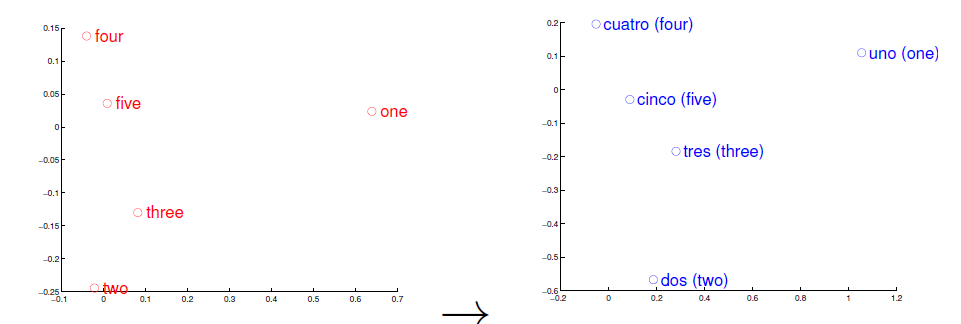
\includegraphics[width=13cm,height=5cm]{2_1}
            \caption{词向量在空间中的映射}
        \end{center}
    \end{figure}

    \section{CBOW模型}
    \subsection{CBOW模型介绍}
    CBOW模型很像 feedforward NNLM(\href{http://jmlr.org/papers/volume3/bengio03a/bengio03a.pdf}{A Neural Probabilistic Language Model}),
    feedforward NNLM模型如下所示:
    \begin{figure}[h]
        \begin{center}
            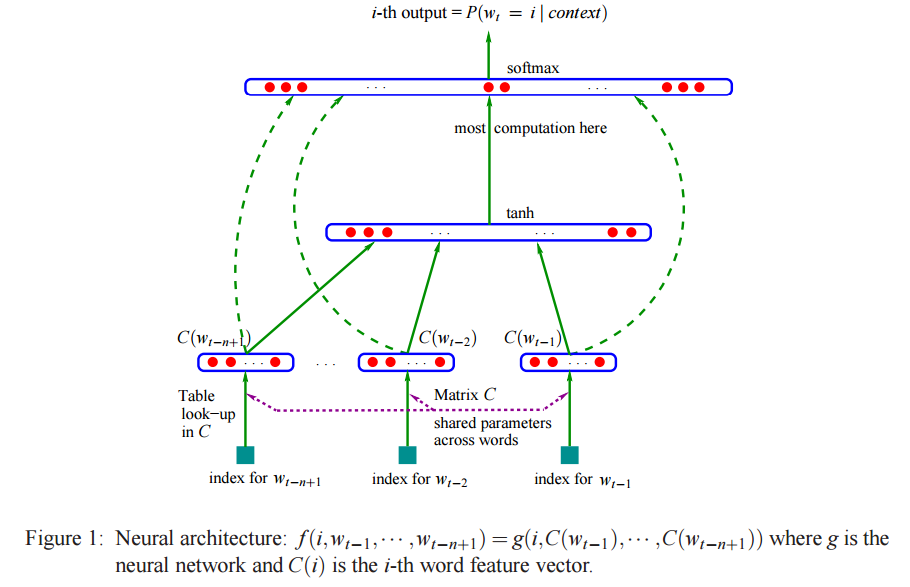
\includegraphics[width=13cm,height=8cm]{2_2}
            \caption{feedforward NNLM模型}
        \end{center}
    \end{figure}

    其中C是一个词向量矩阵,首先,将词$w_i$的词向量从C中取出,
    并且首尾相接组成$\boldsymbol{x}$作为神经网络的第一层输入层,第二层为隐藏层,
    通过 $d+Hx$ 计算得到。$d$ 是一个偏置项。在此之后,使用 $\tanh$ 作为激活函。
    第三层输出层,一共有 $|V|$ 个节点,每个节点 $y_i$ 表示下一个词为$i$的未归一化 
    log 概率。最后使用 softmax 激活函数将输出值 
    $y$ 归一化成概率。最终,$y$ 的计算公式为:$y = b + Wx + U\tanh(d+Hx)$。


    CBOW将隐藏层移除,投影层不再是词向量的拼接,而是各个词向量相加后取平均作为输入,
    由上图可以看到,NNLM模型大部分的计算量在输出层上的softmax归一化运算,
    因此,CBOW为了简化模型,在输出层输出huffman树。CBOW模型根据上下文预测当前词。
    Skip-gram模型是用每个当前词去预测一定范围内除当前词之外前后的词。
    并不是有些人说的CBOW的相反版本。论文关于这一点的原文是:
    \textbf{we use each current word as an input to a log-linear classifier with continuous projection layer, and predict words within a certain range before and after the current word.} 
    \href{http://arxiv.org/pdf/1301.3781v3.pdf}{原文pdf}

    \begin{figure}[h]
        \begin{center}
            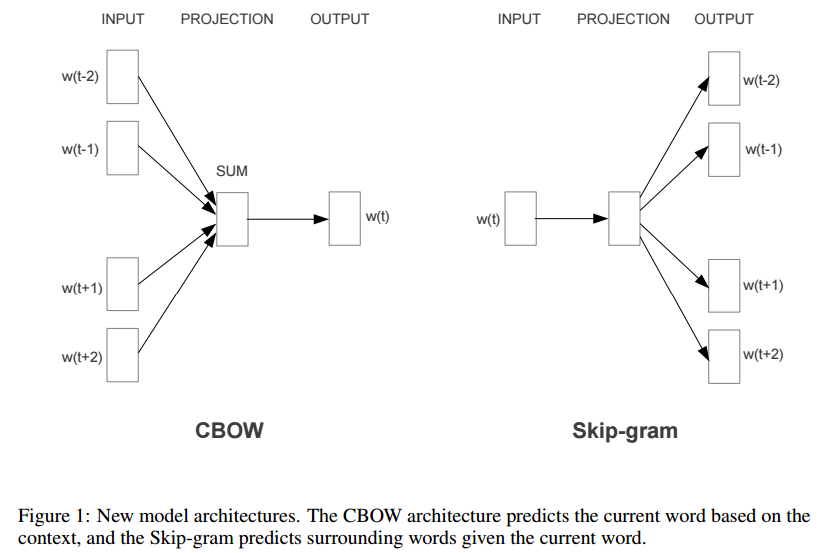
\includegraphics[width=12cm,height=8cm]{2_3}
            \caption{CBOW模型和Skip-gram模型}
        \end{center}
    \end{figure}

    \subsection{CBOW模型的推导}
    由于模型的输出是一颗huffman树,其中树的叶子节点表示词,
    根节点表示权值。
    CBOW的核心内容是推导出$p(w|context(w))$,其中,$context(w)$由w前后各c个词组成。
    如下图所示:下图借用
    \href{http://blog.csdn.net/itplus/article/details/37969979}{基于 Hierarchical Softmax 的模型}.

    \begin{figure}[h]
        \begin{center}
            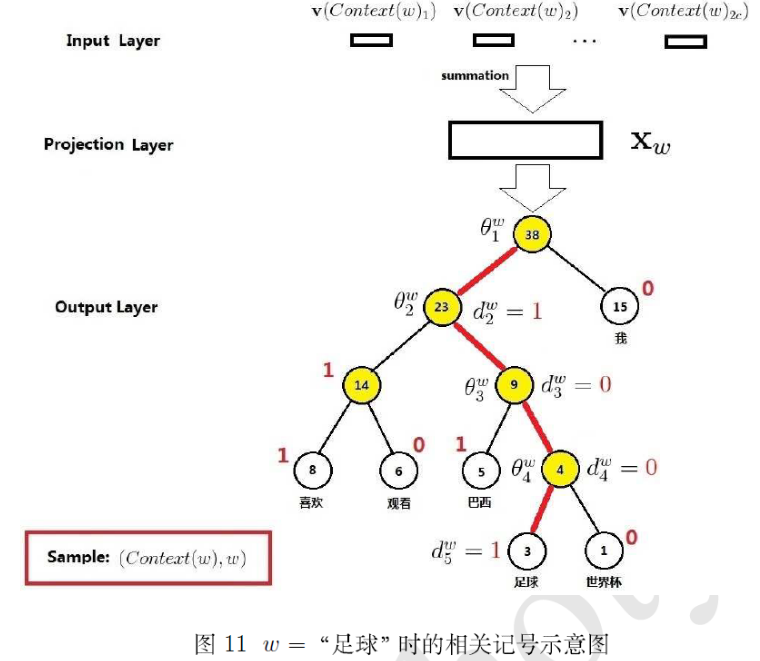
\includegraphics[width=12cm,height=13cm]{2_4}
            \caption{CBOW模型示意图}
        \end{center}
    \end{figure}

    \begin{enumerate}
        \item 由输入层$context(w)$得到投影层向量$\boldsymbol{X_w}$:
        \begin{equation}
            \boldsymbol{X_w} = \sum_{i=1}^{2c} \boldsymbol{V}(context(w)_i)
        \end{equation}
        以上$\boldsymbol{V}(context(w)_i)$初始化为$[\frac{-0.5}{M},\frac{0.5}{M}]$,M为向量的维数。
        \item 由huffman树的根节点到叶节点,是多个二分类问题。二分类问题一般用logistic回归解决,给出回归函数:
        \begin{equation}
            \sigma(z_i) = \frac{1}{1+e^{-z_i}},
        \end{equation} 
        其中,$z=\boldsymbol{X_w^T\theta}$, 
        则
        \begin{equation}
            \Bigg\{ 
                \begin{array} {ll}
                    p(d_i^w|\boldsymbol{X_w^T;\theta_{i-1}})=1-\sigma(z) &, d=1\\
                    p(d_i^w|\boldsymbol{X_w^T;\theta_{i-1}})=\sigma(z) &, d=0
                \end{array}
        \end{equation}

        \item 由以上huffman树的图可知:
        \begin{equation}
            p(w|context(w))=\prod_{i=2}^{l^w} p(d_i^w|\boldsymbol{X_w;\theta_{i-1}})=\prod_{i=2}^{l^w}[\sigma(z_{i-1})^{1-d_i^w}(1-\sigma(z_{i-1}))^{d_i^w}]
        \end{equation}
        \item 语言模型的目标函数是取如下最大似然函数
        \begin{equation}
            \begin{split}
                \mathcal{L}&=\sum_{w \in  \mathcal{C}} \log p(w|context(w))\\
                &=\sum_{w \in  \mathcal{C}} \log \prod_{i=2}^{l^w}[\sigma(z_{i-1})^{1-d_i^w}(1-\sigma(z_{i-1}))^{d_i}]\\
                &=\sum_{w \in  \mathcal{C}}\sum_{i=2}^{l^w}[(1-d_i^w)\log\sigma(z_{i-1})+d_i^w \log (1-\sigma(z_{i-1}))]
            \end{split}
        \end{equation}
        记以下函数为:
        \begin{equation}
            \mathcal{L}(w, i) = (1-d_i^w)\log\sigma(z_{i-1})+d_i^w \log (1-\sigma(z_{i-1})) \\
        \end{equation}
        将$z_i$代入得:
        \begin{equation}
            \mathcal{L}(w, i) = (1-d_i^w)\log\sigma(\boldsymbol{X_w^T\theta_{i-1}})+d_i^w \log (1-\sigma(\boldsymbol{X_w^T\theta_{i-1}})
        \end{equation}
        
        \item 求函数$\mathcal{L}(w, i)$对$w$和$\theta_{i-1}$求偏导数:
        \begin{equation}
            \frac{\partial \mathcal{L}(w, i)}{\partial \boldsymbol{X_w}} = (1-d_i^w-\frac{1}{1+e^{\boldsymbol{-X_w^T\theta_i-1}}})\boldsymbol{\theta_{i-1}}
        \end{equation}
        \begin{equation}
            \frac{\partial \mathcal{L}(w, i)}{\partial \boldsymbol{\theta_{i-1}}} = (1-d_i^w-\frac{1}{1+e^{\boldsymbol{-X_w^T\theta_i-1}}})\boldsymbol{X_w^T}
        \end{equation}

        \item 那么,参数$\theta_{i-1}$的更新公式如下所示:
        \begin{equation}
            \theta_{i-1} := \theta_{i-1} + \eta (1-d_i^w-\frac{1}{1+e^{\boldsymbol{-X_w^T\theta_i-1}}})\boldsymbol{X_w^T}
        \end{equation}
        我们的目的是求每个词的词向量,那么,给出词向量的更新公式:对于每个$w \in context(w)$,都有:
        \begin{equation}
            v(w):=v(w)+\eta \sum_{i=2}^{l_w}(1-d_i^w-\frac{1}{1+e^{\boldsymbol{-X_w^T\theta_i-1}}})\boldsymbol{\theta_{i-1}}
        \end{equation}
    \end{enumerate}

    \section{Skip-gram模型}
    \subsection{Skip-gram模型介绍}
    Skip-gram模型并不是和CBOW模型相反的,
    它们的目的都是计算出词的向量,只不过在作者的论文中给出的图看样子是反的而已。
    Skip-gram模型是用每个当前词去预测一定范围内除当前词之外前后的词。
    同样的,此模型也是输出一颗huffman树,如下图所示:
    \begin{figure}[h]
        \begin{center}
            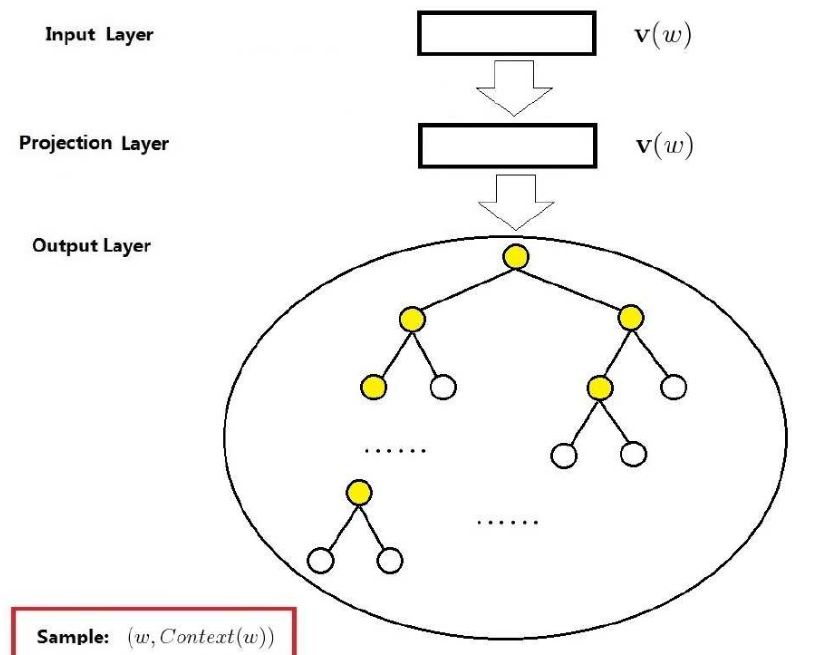
\includegraphics[width=12cm,height=13cm]{3_1}
            \caption{huffman树}
        \end{center}
    \end{figure}
    此图也借用下图借用 
    \href{http://blog.csdn.net/itplus/article/details/37969979}{基于 Hierarchical Softmax 的模型}

    \subsection{Skip-gram模型的目标函数}
    由于Skip-gram的模型输入是当前词,目的是预测它周围的词,因此,此任务的目标函数如下所示:
    \begin{equation}
        \mathcal{L} = \sum_{w \in C} \log P(context(w)|w)
    \end{equation}

    由于$context(w)$ 是一个句子,因此,可以将$P(context(w)|w)$写成如下形式:
    \begin{equation}
        P(context(w)|w) = \prod_{u \in context(w)}P(u|w)
    \end{equation}
    根据hierarchical softmax的讨论:
    \begin{equation}
        P(u|w) = \prod_{j=2}^{l^u}P(d_j^u|v(u); \theta_{j-1})
    \end{equation}
    那么:最终的目标函数可以写为:
    \begin{equation}
        \mathcal{L} = \sum_{w \in C} \log \prod_{u \in context(w)} \prod_{j=2}^{l^u}P(d_j^w|v(u); \theta_{j-1})
    \end{equation}

    \subsection{Skip-gram模型的推导过程}
    \begin{equation}
        \begin{split}
            \mathcal{L} &= \sum_{w \in C} \log \prod_{u \in context(w)} \prod_{j=2}^{l^u}P(d_j^w|v(u); \theta_{j-1}) \\
            &= \sum_{w \in C}\sum_{u \in context(w)} \sum_{j=2}^{l^u} \log P(d_j^w|v(u); \theta_{j-1})\\
            &= \sum_{w \in C}\sum_{u \in context(w)} \sum_{j=2}^{l^u} \log \{ [1-\sigma(v(w)^T\theta_{j-1}^{u})]^{d_j^u} \sigma(v(w)^T\theta_{j-1}^{u})]^{1-d_j^u} \}\\
            &=\sum_{w \in C}\sum_{u \in context(w)} \sum_{j=2}^{l^u} \{d_j^u\log [1-\sigma(v(w)^T\theta_{j-1}^{u})] + (1-d_j^u)\log [\sigma(v(w)^T\theta_{j-1}^{u})]\}
        \end{split}
    \end{equation}

    令
    \begin{equation}
        f = d_j^u\log [1-\sigma(v(w)^T\theta_{j-1}^{u})] + (1-d_j^u)\log [\sigma(v(w)^T\theta_{j-1}^{u})]
    \end{equation}
    则分别求出$f$对$\theta_j$ 和$v(w)$求偏导数:
    \begin{equation}
        \frac{\partial{f}}{\partial{\theta_{j-1}^{u}}}=[1-d_j^u-\sigma(v(w)^T\theta_{j-1}^{u})] v(w)
    \end{equation}
    \begin{equation}
        \frac{\partial{f}}{\partial{v(w)}} = [1-d_j^u-\sigma(v(w)^T\theta_{j-1}^{u})] \theta_{j-1}^{u}
    \end{equation}

    那么$\theta$和$v(w)$的更新公式如下:
    \begin{equation}
        \theta_{j-1}^{u} :=\theta_{j-1}^{u}+\eta [1-d_j^u-\sigma(v(w)^T\theta_{j-1}^{u})] v(w)
    \end{equation}
    \begin{equation}
        v(w):=v(w)+\sum_{u \in context(w)} \sum_{j=2}^{l^u}[1-d_j^u-\sigma(v(w)^T\theta_{j-1}^{u})] \theta_{j-1}^{u}
    \end{equation}


    \section{Word2Vec 的重点参考文献}
    \begin{enumerate}
        \item \href{http://arxiv.org/pdf/1301.3781v3.pdf}{Efficient Estimation of Word Representations in Vector Spaceh. }
        \item \href{https://papers.nips.cc/paper/5021-distributed-representations-of-words-and-phrases-and-their-compositionality.pdf}{Distributed Representations ofWords and Phrases and their Compositionality}
        \item \href{http://static.googleusercontent.com/media/research.google.com/zh-CN//pubs/archive/44931.pdf}{Exploiting Similarities among Languages for Machine Translation }
        \item \href{http://blog.csdn.net/itplus/article/details/37969979}{基于 Hierarchical Softmax 的模型}
        \item \href{http://www.cnblogs.com/neopenx/p/4571996.html}{Word2Vec源码解析}
        \item \href{http://blog.csdn.net/zhoubl668/article/details/24319529}{word2vec中关于霍夫曼树的应用原理}
    \end{enumerate}




    \chapter{Negative Sampling模型}

在负采样中,对于给定的词$w$,如何生成它的负采样集合$NEG(w)$呢?
已知一个词$w$,它的上下文是$context(w)$,那么词$w$就是一个正例,
其他词就是一个负例。但是负例样本太多了,我们怎么去选取呢?
在语料库$\mathcal{C}$中,各个词出现的频率是不一样的,
我们采样的时候要求高频词选中的概率较大,而低频词选中的概率较小。
这就是一个带权采样的问题。
设词典$\mathcal{D}$中的每一个词$w$对应线段的一个长度:
\begin{equation}
    len(w) = \frac{counter(w)}{\sum_{u \in \mathcal{D}}counter(u)} (1)
\end{equation}
式4.1分母是为了归一化,Word2Vec中的具体做法是:
记$l_0 = 0, l_k = \sum_{j=1}^{k} len(w_j), k=1,2, \dots, N$,
其中,$w_j$是词典$\mathcal{D}$中的第$j$个词,
则以$\{l_j\}_{j=0}^{N}$为点构成了一个在区间[0,1]非等距离的划分。
然后再加一个等距离划分,Word2Vec中选取$M=10^8$,将M个点等距离的分布在区间[0,1]上,
这样就构成了M到I之间的一个映射,如下图所示:
\begin{figure}[h]
    \begin{center}
        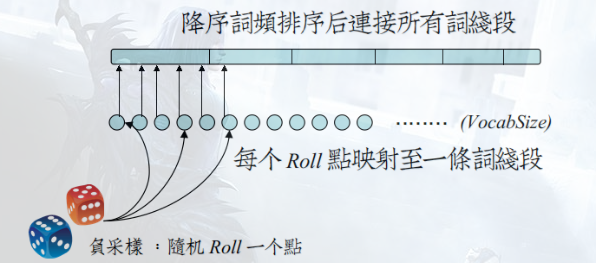
\includegraphics[width=12cm, height=6cm]{4_1}
        \caption{负采样}
    \end{center}
\end{figure}

图例参考:
\href{http://www.cnblogs.com/neopenx/p/4571996.html}{\textbf{建议大家读下这篇神作}}。

选取负例样本的时候,取$[M_0, M_{m-1}]$上的一个随机数,对应到I上就可以了。
如果对于词$w_i$,正好选到它自己,则跳过。负例样本集合$NEG(w)$的大小在Word2Vec源码中默认选5.

\section{CBOW}
假定关于词$w$的负例样本$NEG(w)$已经选出,定义标签$L$如下,
对于 $\forall \widetilde{w} \in \mathcal{D}$:
\begin{equation}
    L^w(\widetilde{w}) = \Bigg\{ \begin{array} {ll}
        1,  & \widetilde{w} = w ;\\
        0, & \widetilde{w} \ne w;
        \end{array}
\end{equation}

对于给定的一个正例样本$(context(w), w)$, 要求:
\begin{equation}
    \max g(w) = \max \prod_{u \in \{w\} \cup u \in NEG(w)} p(u|context(w))
\end{equation}

其中, 
\begin{equation}
    p(u|context(w)) = \Bigg \{ \begin{array}{ll}
        \sigma(\boldsymbol{x}_w^T \theta^u), & L^w(u) = 1\\
        1-\sigma(\boldsymbol{x}_w^T \theta^u), & L^w(u) = 0
        \end{array}
\end{equation}

把它写成一个式子:
\begin{equation}
    p(u|context(w)) = \sigma(\boldsymbol{x}_w^T \theta^u)^{L^w(u)} + (1-\sigma(\boldsymbol{x}_w^T \theta^u))^{1-L^w(u)}
\end{equation}

下边解释为什么要最大化$g(w)$,
\begin{equation}
    \begin{split}
        g(w) &= \prod_{u \in \{w\} \cup u \in NEG(w)} p(u|context(w)) \\
        &=\prod_{u \in \{w\} \cup u \in NEG(w)}  \sigma(\boldsymbol{x}_w^T \theta^u)^{L^w(u)} + (1-\sigma(\boldsymbol{x}_w^T \theta^u))^{1-L^w(u)} \\ 
        &=\sigma(\boldsymbol{x}_w^T \theta^w)\prod_{u \in NEG(w)} (1-\sigma(\boldsymbol{x}_w^T \theta^u))
    \end{split}
\end{equation}

\textbf{上式中连乘号前边的式子可以解释为最大化正例样本概率,连乘号后边解释为最小化负例样本概率}。

同样的,针对于语料库,令:
\begin{equation}
    \mathcal{G} = \prod_{w \in \mathcal{C}} g(w)
\end{equation}

可以将上式作为整体的优化目标函数,取上式的最大似然:
\begin{equation}
    \begin{split}
    \mathcal{L} = \log\mathcal{G} \\
    &= \sum_{w \in \mathcal{C}} \log g(w) \\
    &=\sum_{w \in \mathcal{C}} \sum_{u \in \{w\} \cup u \in NEG(w)}L^w(u)\log[\sigma(\boldsymbol{x}_w^T \boldsymbol{\theta}^u] + [1-L^w(u)]
    \log [1-\sigma(\boldsymbol{x}_w^T \boldsymbol{\theta}^u)]
\end{split}
\end{equation}

和之前的计算过程一样,记
\begin{equation}
    L(w,u) = L^w(u)\log[\sigma(\boldsymbol{x}_w^T \theta^u] + [1-L^w(u)]\log [1-\sigma(\boldsymbol{x}_w^T \boldsymbol{\theta}^u)]
\end{equation}

然后分别求:$\frac{\partial L(w,u)}{\partial\boldsymbol{X}_w}$和$\frac{\partial L(w,u)}{\partial\boldsymbol{\theta}^u}$,求解过程略过:
\begin{equation}
    \frac{\partial L(w,u)}{\partial\boldsymbol{X}_w} = [L^w(u)-\sigma(\boldsymbol{x}_w^T \boldsymbol{\theta}^u)]\boldsymbol{\theta}^u 
\end{equation}
\begin{equation}
    \frac{\partial L(w,u)}{\partial\boldsymbol{\theta}^u} = [L^w(u)-\sigma(\boldsymbol{x}_w^T \boldsymbol{\theta}^u)]\boldsymbol{X}_w
\end{equation}
则,可得到如下更新公式:
\begin{equation}
    \boldsymbol{\theta}^u:=\boldsymbol{\theta}^u+\eta [L^w(u)-\sigma(\boldsymbol{x}_w^T \boldsymbol{\theta}^u)]\boldsymbol{X}_w \\
\end{equation}
\begin{equation}
    v(\boldsymbol{\widetilde{w}}):=v(\boldsymbol{\widetilde{w}}) + \sum_{u \in \{w\} \cup u \in NEG(w)} [L^w(u)-\sigma(\boldsymbol{x}_w^T \boldsymbol{\theta}^u)]\boldsymbol{\theta}^u
\end{equation}
其中, $\boldsymbol{\widetilde{w}} \in context(w)$.

\section{Skip-gram模型}
这部分内容并不多,与cbow相比,只是目标函数有所变化,推导过程这里就略过。
总的来说,就是将目标函数取最大似然,然后利用SGD方法求出词向量和最优参数。
目标函数如下所示:
\begin{equation}
    G = \prod_{w \in \mathcal{C}} g(w)
\end{equation}
其中,$g(w)$可以改写成如下形式:
\begin{equation}
    g(w)=\prod_{u \in context(w)} g(u)
\end{equation}
$g(u)$表示如下:
\begin{equation}
    g(u) = \prod_{z \in \{u\} \cup NEG(u)} p(z|w)
\end{equation}
其中,$NEG(u)$表示在处理词$u$时产生的负样本集合。$p(z|w)$如下:
\begin{equation}
    p(z|w) = \Bigg \{ \begin{array}{ll}
    \sigma(\boldsymbol{v(w)}^T \theta^z), & L^u(z) = 1\\
    1-\sigma(\boldsymbol{v(w)}^T \theta^z), & L^u(z) = 0
    \end{array}
\end{equation}
将以上式子合并之后就可以得到最终的目标函数:
\begin{equation}
    G = \prod_{w \in \mathcal{C}}\prod_{u \in context(w)}\prod_{z \in \{u\} \cup NEG(u)} \sigma(\boldsymbol{v(w)}^T \theta^z)^{L^u(z)}(1-\sigma(\boldsymbol{v(w)}^T \theta^z))^{L^u(z)}
\end{equation}
然后取$G$的最大似然对数,求目标函数的最优化。

 
    \chapter{Word2Vec训练同义词模型}
\section{需求描述}
业务需求的目标是识别出目标词汇的同义词和相关词汇,如下为部分目标词汇(主要用于医疗问诊):
\begin{itemize}
    \item 尿
    \item 痘痘
    \item 发冷
    \item 呼吸困难 
    \item 恶心
\end{itemize}

数据源是若干im数据,那么这里我们选择google 的word2vec模型来训练同义词和相关词。

\section{数据处理}

数据处理考虑以下几个方面:
\begin{enumerate}
    \item 从hive中导出不同数据量的数据
    \item 过滤无用的训练样本(例如字数少于5)
    \item 准备自定义的词汇表
    \item 准备停用词表
\end{enumerate}

\section{工具选择}

选择python 的gensim库,由于先做预研,数据量不是很大,选择单机就好,
暂时不考虑spark训练。后续生产环境计划上spark。
\href{https://radimrehurek.com/gensim/models/word2vec.html}{详细的gensim中word2vec文档}

上述文档有关工具的用法已经很详细了,就不多说。

分词采用jieba。

\section{模型训练步骤简述}
\begin{enumerate}
    \item 先做分词、去停用词处理
    \begin{python}
        seg_word_line = jieba.cut(line, cut_all = True)
    \end{python}
\end{enumerate}
1.
```python

```
2.将分词的结果作为模型的输入
```python
model = gensim.models.Word2Vec(LineSentence(source_separated_words_file), size=200, window=5, min_count=5, alpha=0.02, workers=4)
```
3.保存模型,方便以后调用,获得目标词的同义词
```python
similary_words = model.most_similar(w, topn=10)
```

## 五、重要调参目标

&nbsp;&nbsp;&nbsp;&nbsp; 比较重要的参数:
1. 训练数据的大小,当初只用了10万数据,训练出来的模型很不好,后边不断地将训练语料增加到800万,效果得到了明显的提升
2. 向量的维度,这是词汇向量的维数,这个会影响到计算,理论上来说维数大一点会好。
3. 学习速率
4. 窗口大小

在调参上,并没有花太多精力,因为目测结果还好,到时上线使用前再仔细调整。

## 六、模型的实际效果

| 目标词        | 同义词相关词    | 
| ------------- |:-------------| 
| 尿      | 尿液,撒尿,尿急,尿尿有,尿到,内裤,尿意,小解,前列腺炎,小便 | 
| 痘痘      | 逗逗,豆豆,痘子,小痘,青春痘,红痘,长痘痘,粉刺,讽刺,白头     |   
| 发冷 | 发烫,没力,忽冷忽热,时冷时热,小柴胡,头昏,嗜睡,38.9,头晕,发寒      |   
| 呼吸困难 | 气来,气紧,窒息,大气,透不过气,出不上,濒死,粗气,压气,心律不齐     |   
| 恶心 | 闷,力气,呕心,胀气,涨,不好受,不进,晕车,闷闷,精神|   

## 七、可以跑的CODE

```python
import codecs
import jieba
import gensim
from gensim.models.word2vec import LineSentence

def read_source_file(source_file_name):
    try:
        file_reader = codecs.open(source_file_name, 'r', 'utf-8',errors="ignore")
        lines = file_reader.readlines()
        print("Read complete!")
        file_reader.close()
        return lines
    except:
        print("There are some errors while reading.")

def write_file(target_file_name, content):
    
    file_write = codecs.open(target_file_name, 'w+', 'utf-8')
    file_write.writelines(content)
    print("Write sussfully!")
    file_write.close()

def separate_word(filename,user_dic_file, separated_file):
    print("separate_word")
    lines = read_source_file(filename)
    #jieba.load_userdict(user_dic_file)
    stopkey=[line.strip() for line in codecs.open('stopword_zh.txt','r','utf-8').readlines()]

    output = codecs.open(separated_file, 'w', 'utf-8')
    num = 0
    for line in lines:
        num = num + 1
        if num% 10000 == 0:
            print("Processing line number: " + str(num))
        seg_word_line = jieba.cut(line, cut_all = True)
        wordls = list(set(seg_word_line)-set(stopkey))
        if len(wordls)>0:
            word_line = ' '.join(wordls) + '\n'
        output.write(word_line)
    output.close()
    return separated_file
   

def build_model(source_separated_words_file,model_path):

    print("start building...",source_separated_words_file)
    model = gensim.models.Word2Vec(LineSentence(source_separated_words_file), size=200, window=5, min_count=5, alpha=0.02, workers=4)       
    model.save(model_path)
    print("build successful!", model_path)
    return model

def get_similar_words_str(w, model, topn = 10):
    result_words = get_similar_words_list(w, model)    
    return str(result_words)


def get_similar_words_list(w, model, topn = 10):
    result_words = []
    try:
        similary_words = model.most_similar(w, topn=10)
        print(similary_words)
        for (word, similarity) in similary_words:
            result_words.append(word)
        print(result_words)
    except:
        print("There are some errors!" + w)
        
    return result_words

def load_models(model_path):
    return gensim.models.Word2Vec.load(model_path)

if "__name__ == __main__()":
    filename = "d:\\data\\dk_mainsuit_800w.txt" #source file
    user_dic_file = "new_dict.txt" # user dic file
    separated_file = "d:\\data\\dk_spe_file_20170216.txt" # separeted words file
    model_path = "information_model0830" # model file
    
    #source_separated_words_file = separate_word(filename, user_dic_file, separated_file)
    source_separated_words_file = separated_file    # if separated word file exist, don't separate_word again
    build_model(source_separated_words_file, model_path)# if model file is exist, don't buile modl 

    model = load_models(model_path)
    words = get_similar_words_str('头痛', model)
    print(words)

```
    \chapter{next}

\end{CJK*}
\end{document}
